\documentclass[a4paper,12pt]{article}

\usepackage[T2A]{fontenc}			
\usepackage[utf8]{inputenc}			
\usepackage[english,russian]{babel}	

\usepackage[
bookmarks=true, colorlinks=true, unicode=true,
urlcolor=black,linkcolor=black, anchorcolor=black,
citecolor=black, menucolor=black, filecolor=black,
]{hyperref}

\usepackage{color}
\usepackage{caption}
\DeclareCaptionFont{white}{\color{black}}
\DeclareCaptionFormat{listing}{\colorbox{white}{\parbox{\textwidth}{#1#2#3}}}
\captionsetup[lstlisting]{format=listing,labelfont=white,textfont=white}

\usepackage{amsmath,amsfonts,amssymb,amsthm,mathtools} 
\usepackage{wasysym}

\usepackage{graphicx}
%\usepackage[cache=false]{minted}
\usepackage{cmap}
\usepackage{indentfirst}

\usepackage{listings} 
\usepackage{fancyvrb}

\usepackage{geometry}
\geometry{left=2cm}
\geometry{right=1.5cm}
\geometry{top=1cm}
\geometry{bottom=2cm}

\usepackage[cache=false]{minted}

\setlength{\parindent}{5ex}
\setlength{\parskip}{0.5em}

\usepackage{pgfplots}
\usetikzlibrary{datavisualization}
\usetikzlibrary{datavisualization.formats.functions}

\begin{document}

	\lstset{ %
		language=C,                 % выбор языка для подсветки (здесь это С)
		basicstyle=\small\sffamily, % размер и начертание шрифта для подсветки кода
		numbers=left,               % где поставить нумерацию строк (слева\справа)
		numberstyle=\tiny,           % размер шрифта для номеров строк
		stepnumber=1,                   % размер шага между двумя номерами строк
		numbersep=5pt,                % как далеко отстоят номера строк от подсвечиваемого кода
		backgroundcolor=\color{white}, % цвет фона подсветки - используем \usepackage{color}
		showspaces=false,            % показывать или нет пробелы специальными отступами
		showstringspaces=false,      % показывать или нет пробелы в строках
		showtabs=false,             % показывать или нет табуляцию в строках
		frame=single,              % рисовать рамку вокруг кода
		tabsize=2,                 % размер табуляции по умолчанию равен 2 пробелам
		captionpos=t,              % позиция заголовка вверху [t] или внизу [b] 
		breaklines=true,           % автоматически переносить строки (да\нет)
		breakatwhitespace=false, % переносить строки только если есть пробел
		escapeinside={\%*}{*)}   % если нужно добавить комментарии в коде
	}
	
	% Титульный лист
	\begin{figure}[h!]
		\begin{center}
			{
\includegraphics[scale = 0.4]{titul.jpg}}
			\label{titul}
		\end{center}
	\end{figure}
	
	\vspace*{15mm} 
	
	\huge
	\begin{center}
		Дисциплина: <<Операционные системы>>
	\end{center}
	
	\begin{center}
		Лабораторная работа №3
	\end{center}

	
	\huge
	\begin{center}
		Тема работы:\\
		<<Загружаемые модули ядра>>
	\end{center}
	\vspace*{30mm} 
	
	\large
	\begin{flushright}
		Студент: Левушкин И. К. \\
		Группа: ИУ7-62Б \\
		Преподаватель: Рязанова Н. Ю. \\
	\end{flushright}
	
	\vspace*{30mm}
	\begin{center}
		Москва, 2020 г.  
	\end{center}
	\thispagestyle{empty}
	
	\newpage
	
	\section*{Цель работы}
	
	Знакомство с базовыми принципами разработки и взаимодействия с загружаемыми модулями ядра ОС Linux.
	
	\section*{Задание 1}
	
	Реализовать загружаемый модуль ядра, который при загрузке записывает в системный журнал сообщение “Hello world!”, а при выгрузке “Good by”. Модуль должен собираться при помощи Make-файла. 
	Загружаемый модуль должен содержать:
	\begin{itemize}
		\item Указание лицензии GPL
		\item Указание автора
	\end{itemize}

	\newpage

	\section*{Листинг кода программы}
	
	\begin{figure}[h!]
		\begin{center}
			{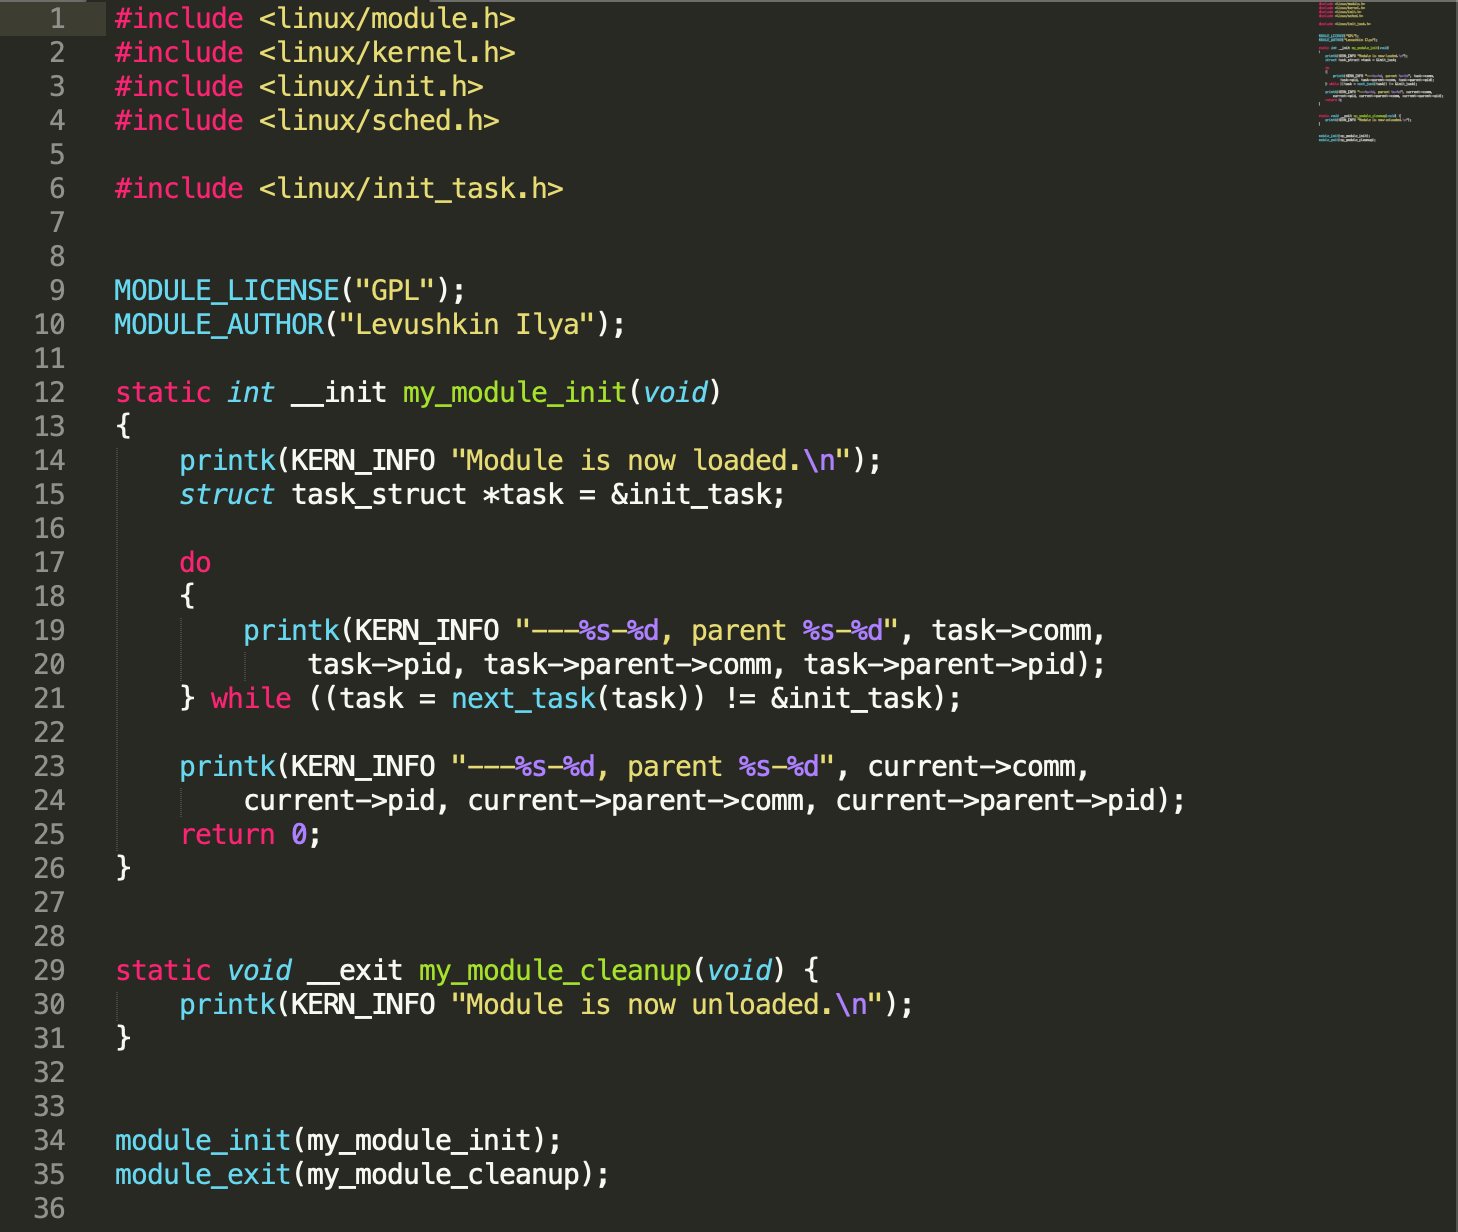
\includegraphics[scale = 0.7]{listing_md.png}}
			\label{listing_md}
		\end{center}
		\caption{md.c}
	\end{figure}
	
	\newpage
	
	\section*{Демонстрация работы программы}
	
	Ниже продемонстрированы загрузка модуля ядра, вывод списка загруженных модулей ядра (команда lsmod), чье название содержит строку <<md>>, последние 20 сообщений, выведенных модулями ядра и информация о модуле.
	
	\begin{figure}[h!]
		\begin{center}
			{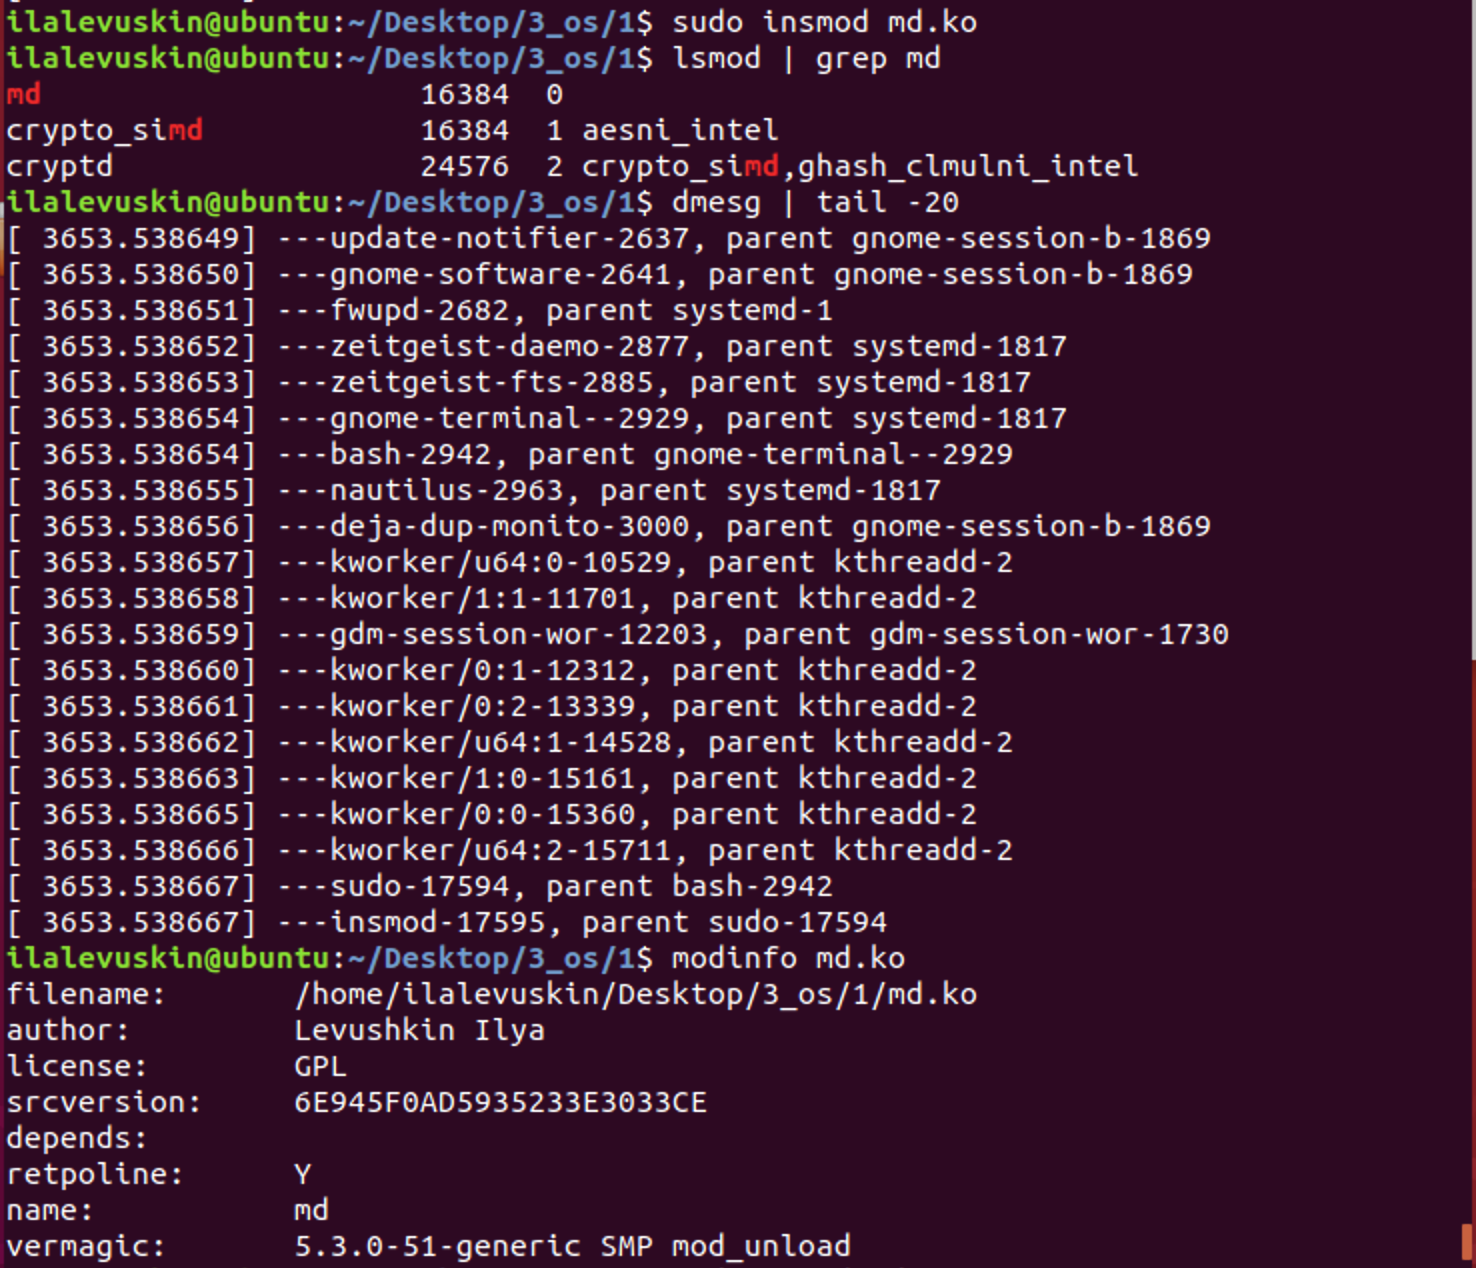
\includegraphics[scale = 0.7]{1.png}}
			\label{1}
		\end{center}
	\end{figure}

	Видно, что модуль успешно загружен.

	\newpage

	Ниже продемонстрированы выгрузка модуля ядра и последние 5 сообщений, выведенных модулями ядра.

	\begin{figure}[h!]
		\begin{center}
			{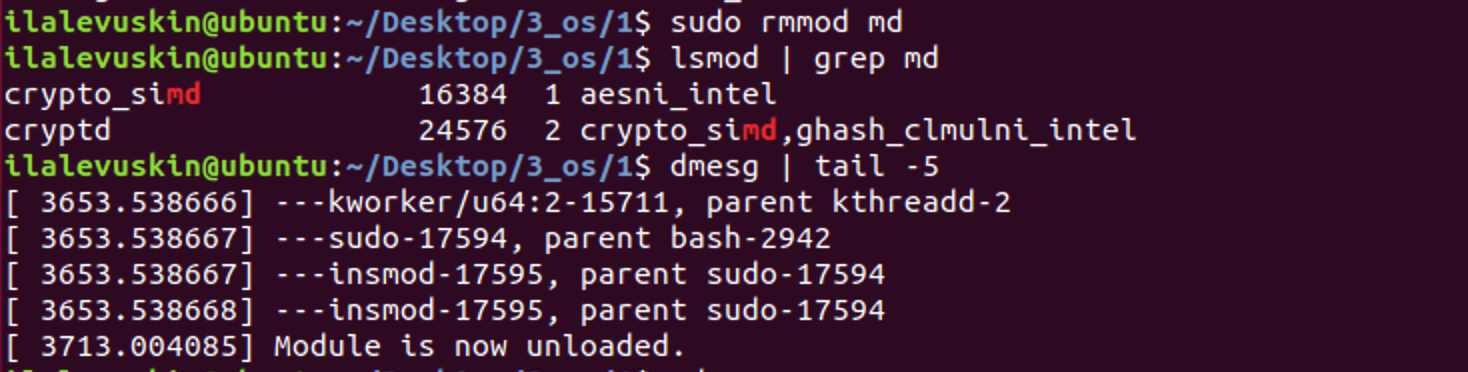
\includegraphics[scale = 0.7]{2.png}}
			\label{2}
		\end{center}
	\end{figure}

	Видно, что модуль успешно выгружен.
	
	
	\section*{Задание 2}
	
	Реализовать три загружаемых модуля ядра:
	\begin{itemize}
		\item Вызываемый модуль md1
		\item Вызывающий модуль md2
		\item <<Отладочный>> модуль md3
	\end{itemize}

	Каждый загружаемый модуль должен содержать:
	\begin{itemize}
		\item Указание лицензии GPL
		\item Указание автора
	\end{itemize}
	Загружаемые модули должны собираться при помощи Make-файла (сборка командой make). {\bf Вызов каждой функции модуля должен сопровождаться записью в системный журнал} информации, какая функция какого модуля была вызвана.
	
	\subsection*{Модуль md1}
	
	Модуль md1 демонстрирует возможность создания экспортируемых данных и  функций.
	
	 Данный модуль ядра должен содержать:
	\begin{itemize}
		\item Экспортируемые строковые (char *) и численные (int) данные.
		\item Экспортируемые функции возвращающие строковые и числовые значения.
	\end{itemize}

	Например:
	\begin{itemize}
		\item Функция, возвращающая в зависимости от переданного целочисленного параметра различные строки (на усмотрение студента);
		\item Функция, производящая подсчет факториала переданного целочисленного параметра;
		\item Функция возвращающая 0; 
	\end{itemize}
	
	
	\subsection*{Модуль md2}
	
	Модуль md2 демонстрирует использование данных и функций экспортируемых первым модулем (md1).
	
	Данный модуль должен при загрузке:
	\begin{itemize}
		\item Вызывать все экспортированные модулем md1 процедуры и вывести в системный журнал возвращаемые ими значения с указанием имени вызванной процедуры.
		\item Вывести в системный журнал все экспортированные модулем md1 данные.
	\end{itemize}
	
	
	\subsection*{Модуль md3}
	
	Модуль md3 демонстрирует сценарий некорректного завершения установки модуля, и возможность использования загружаемого модуля в качестве функции выполняемой в пространстве ядре.  
	
	Процедура инициализации этого загружаемого модуля должна возвращать ненулевое значение и выводить в системный журнал данные и возвращаемые значения экспортированных модулем md1 процедур (аналогично md2).
	
	Данный модуль включен в работу для проработки вопросов, связанных с отладкой модулей ядра. 
	
	\subsection*{Make-файл}
	
	Make-файл должен быть написан так, чтобы при вызове команды make происходила компиляция всех реализованных загружаемых модулей. Это позволит упростить процесс компиляции. Также Make-файл должен содержать правило clean для очистки директории от промежуточных файлов компиляции. 
	
	Пример Make-файла предназначенного для сборки и компиляции загружаемого модуля ядра:
	
	\begin{minted}{makefile}
ifneq ($(KERNELRELEASE),)
	obj-m   := md.o
else
	CURRENT = $(shell uname -r)
	KDIR = /lib/modules/$(CURRENT)/build 
	PWD = $(shell pwd)
default: 
	$(MAKE) -C $(KDIR) M=$(PWD) modules 
clean: 
	@rm -f *.o .*.cmd .*.flags *.mod.c *.order 
	@rm -f .*.*.cmd *~ *.*~ TODO.* 
	@rm -fR .tmp* 
	@rm -rf .tmp_versions 
disclean: clean 
	@rm *.ko *.symvers 

endif
// $(MAKE) - вызов MAKE в режиме ядра. 
	\end{minted}
	
	\newpage
	
	\section*{Листинг кода программы}
	
	\begin{figure}[h!]
		\begin{center}
			{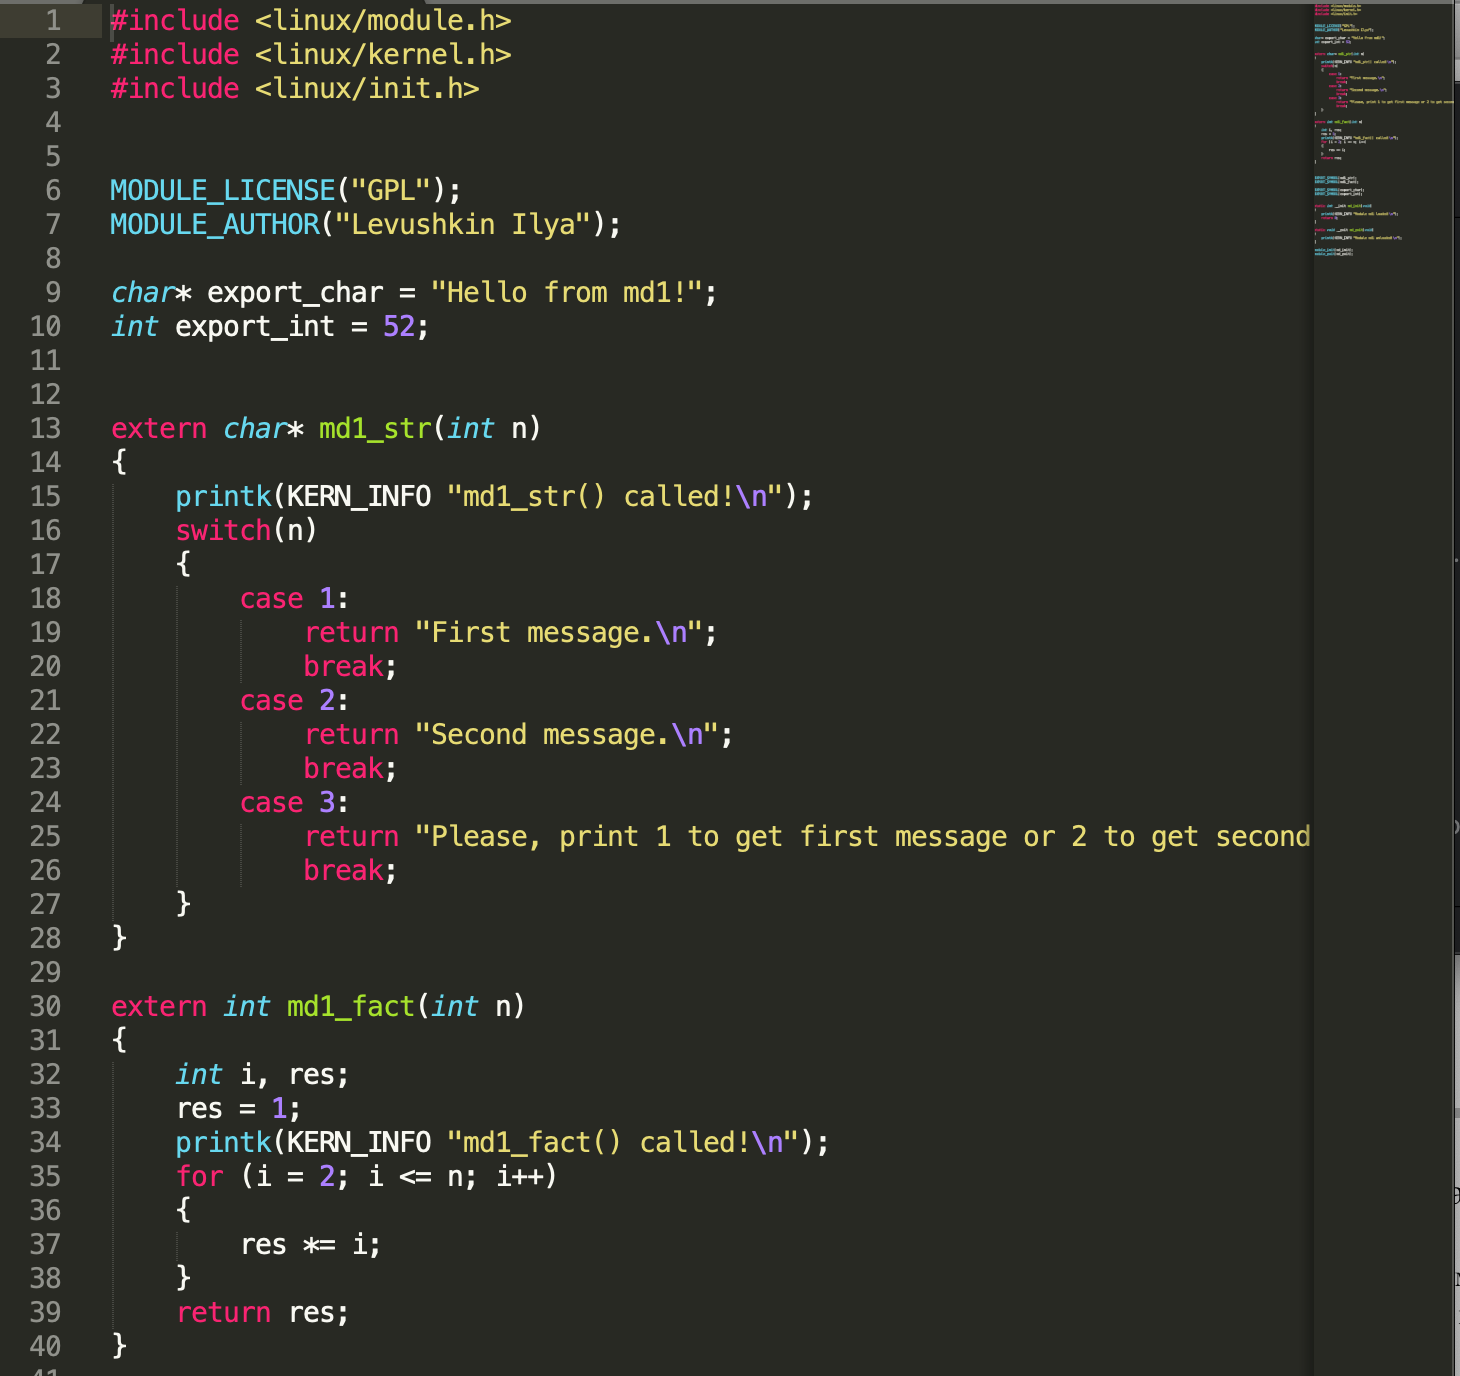
\includegraphics[scale = 0.7]{listing_md1.png}}
			\label{listing_md1}
		\end{center}
		\caption{md1.c}
	\end{figure}

	\newpage

	\begin{figure}[h!]
		\begin{center}
			{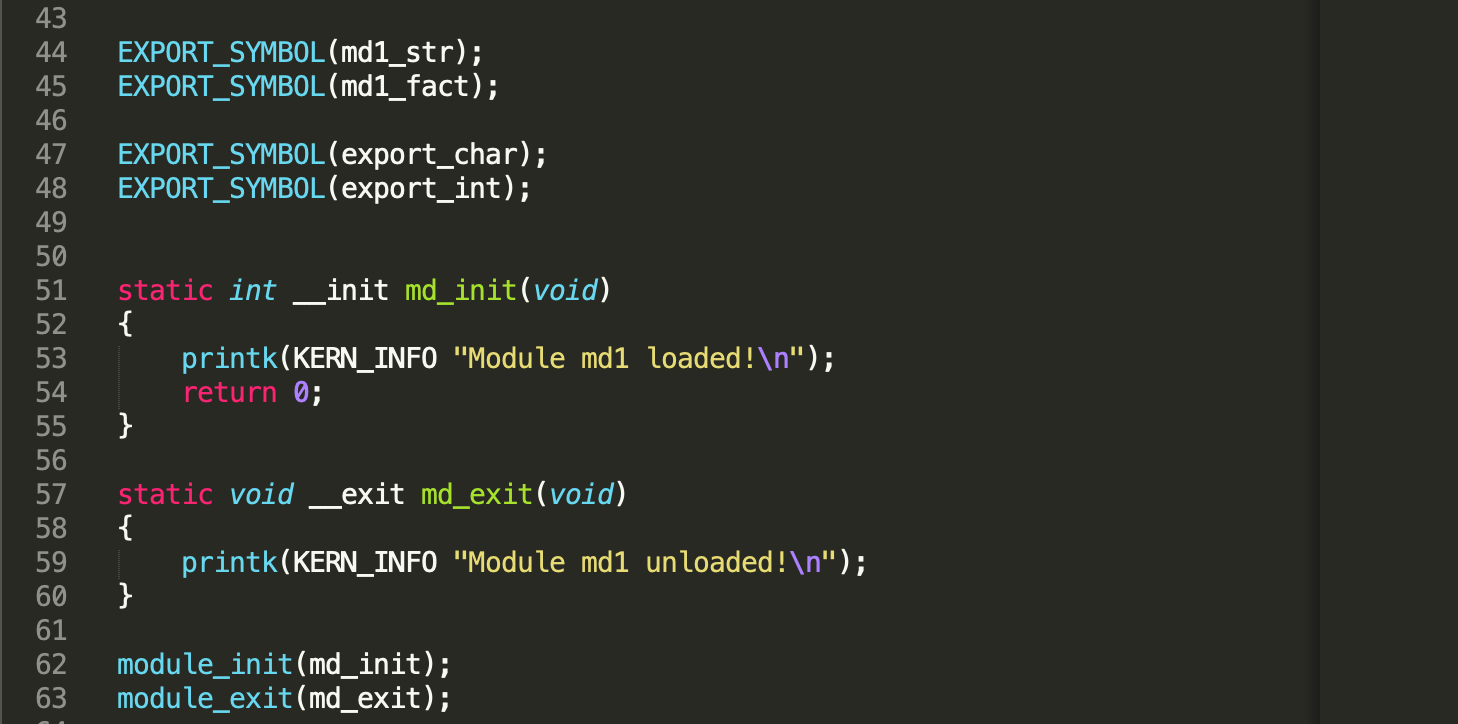
\includegraphics[scale = 0.65]{listing_md1_2.png}}
			\label{listing_md1_2}
		\end{center}
		\caption{md1.c}
	\end{figure}

	\begin{figure}[h!]
		\begin{center}
			{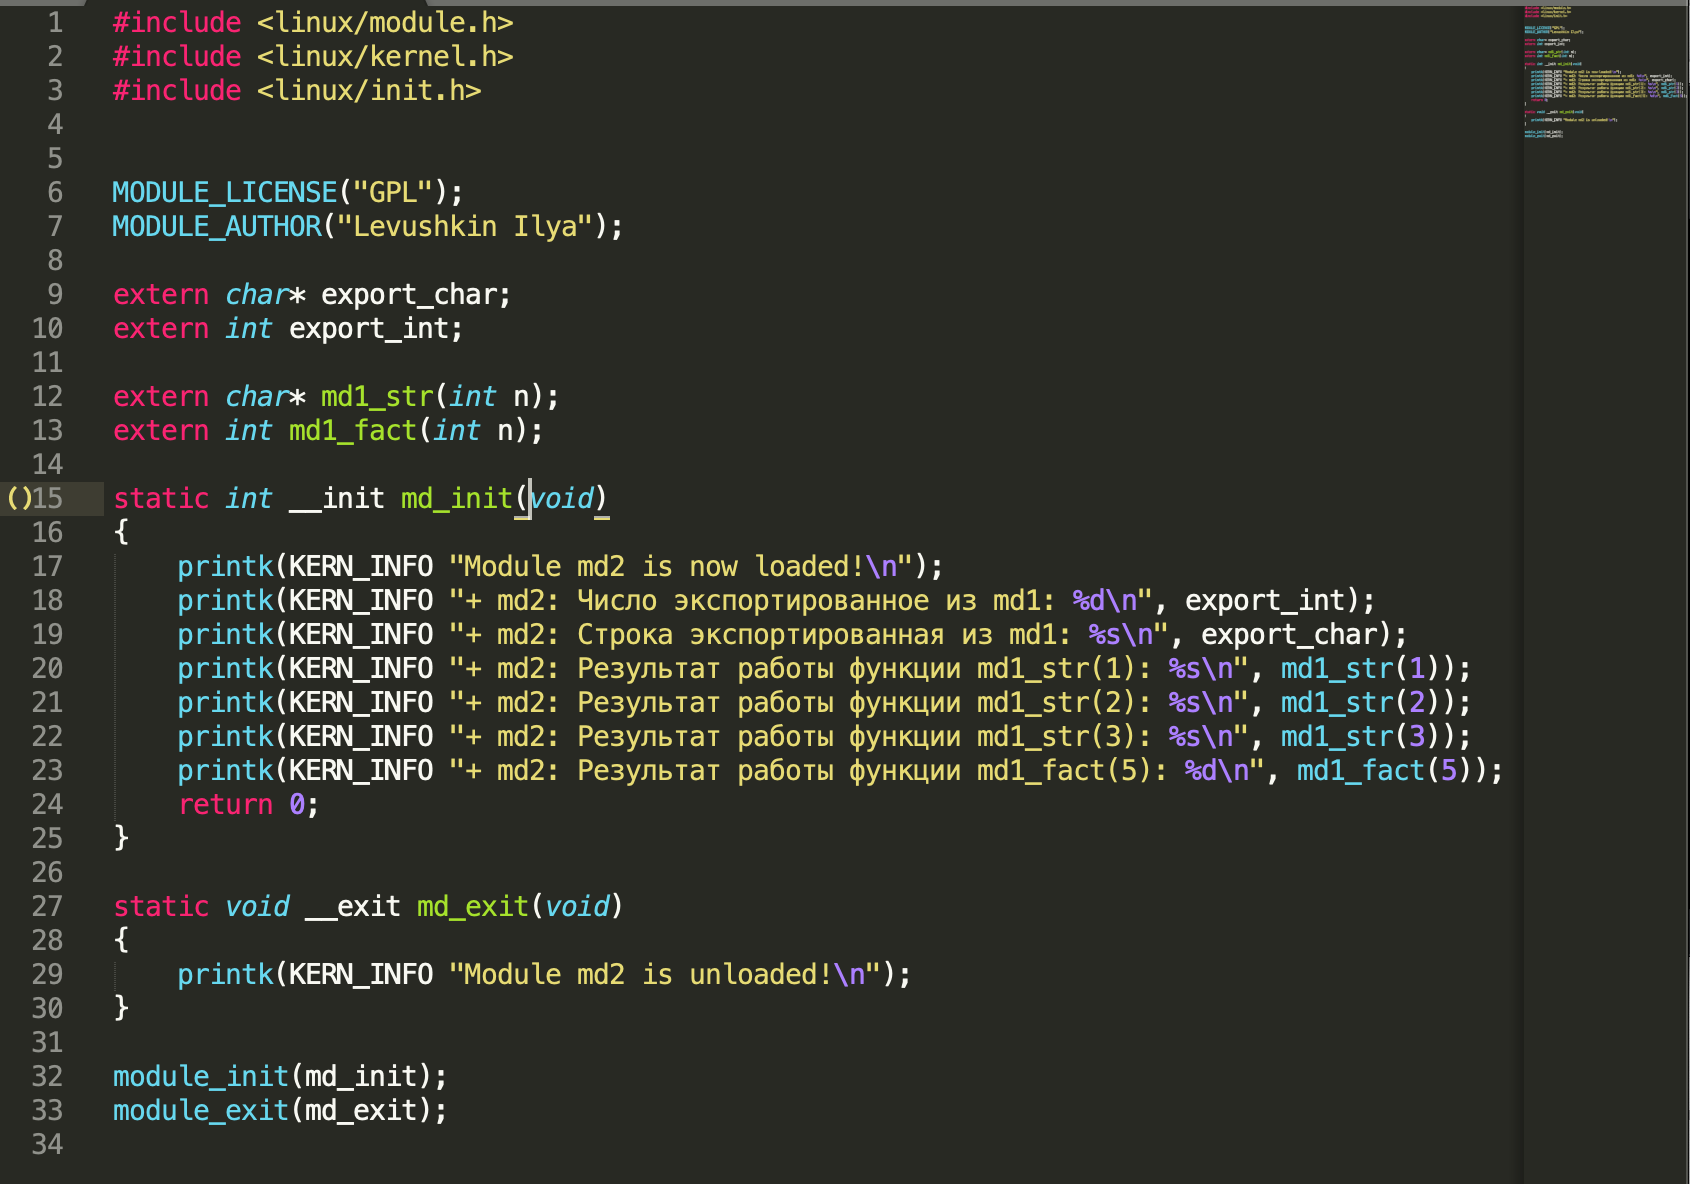
\includegraphics[scale = 0.65]{listing_md2.png}}
			\label{listing_md2}
		\end{center}
		\caption{md2.c}
	\end{figure}

	\newpage

	\begin{figure}[h!]
		\begin{center}
			{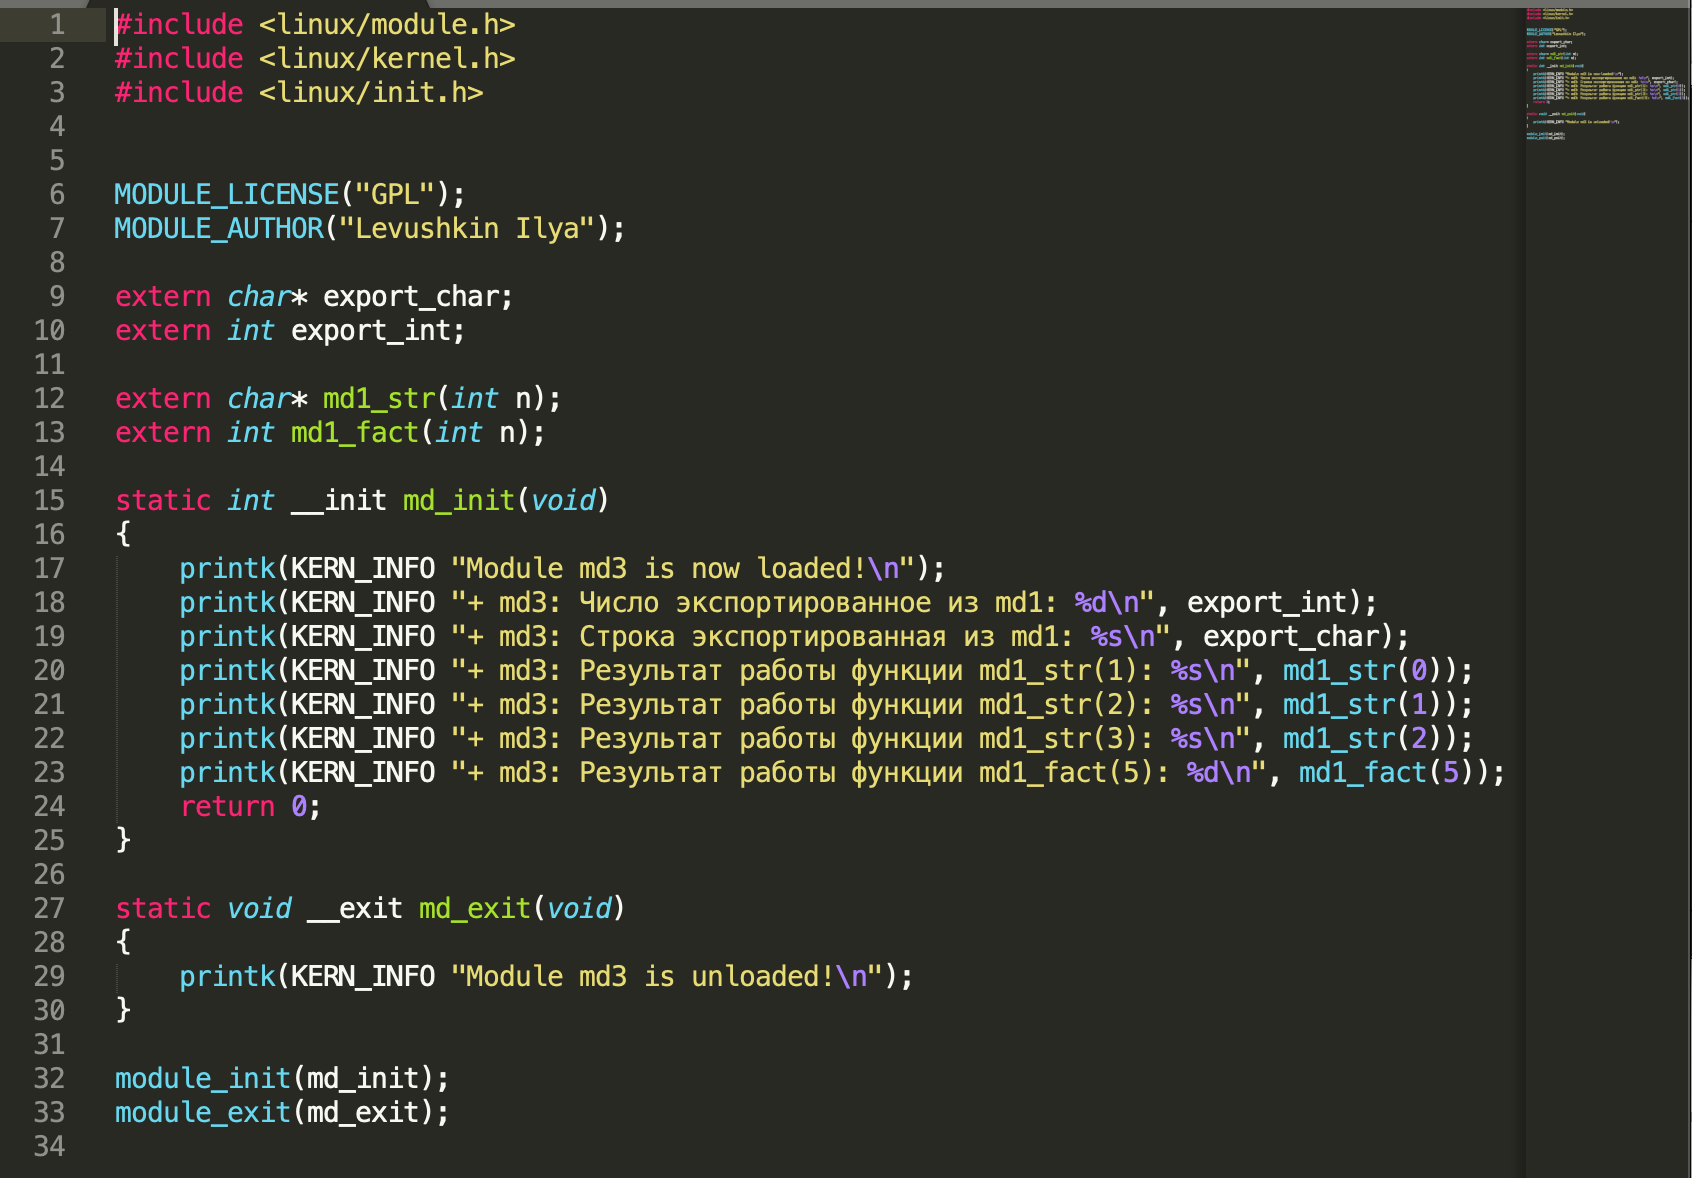
\includegraphics[scale = 0.65]{listing_md3.png}}
			\label{listing_md3}
		\end{center}
		\caption{md3.c}
	\end{figure}

	\newpage
	
	\section*{Демонстрация работы программы}
	
	Ниже продемонстрированы загрузка вначале модуля ядра <<md1>> и вывод списка загруженных модулей ядра (команда lsmod), чье название содержит строку <<md1>>, затем модуля ядра <<md2>> и вывод списка загруженных модулей ядра (команда lsmod), чье название содержит строку <<md2>>, и модуля ядра <<md3>> и вывод списка загруженных модулей ядра (команда lsmod), чье название содержит строку <<md3>>.
	
	\begin{figure}[h!]
		\begin{center}
			{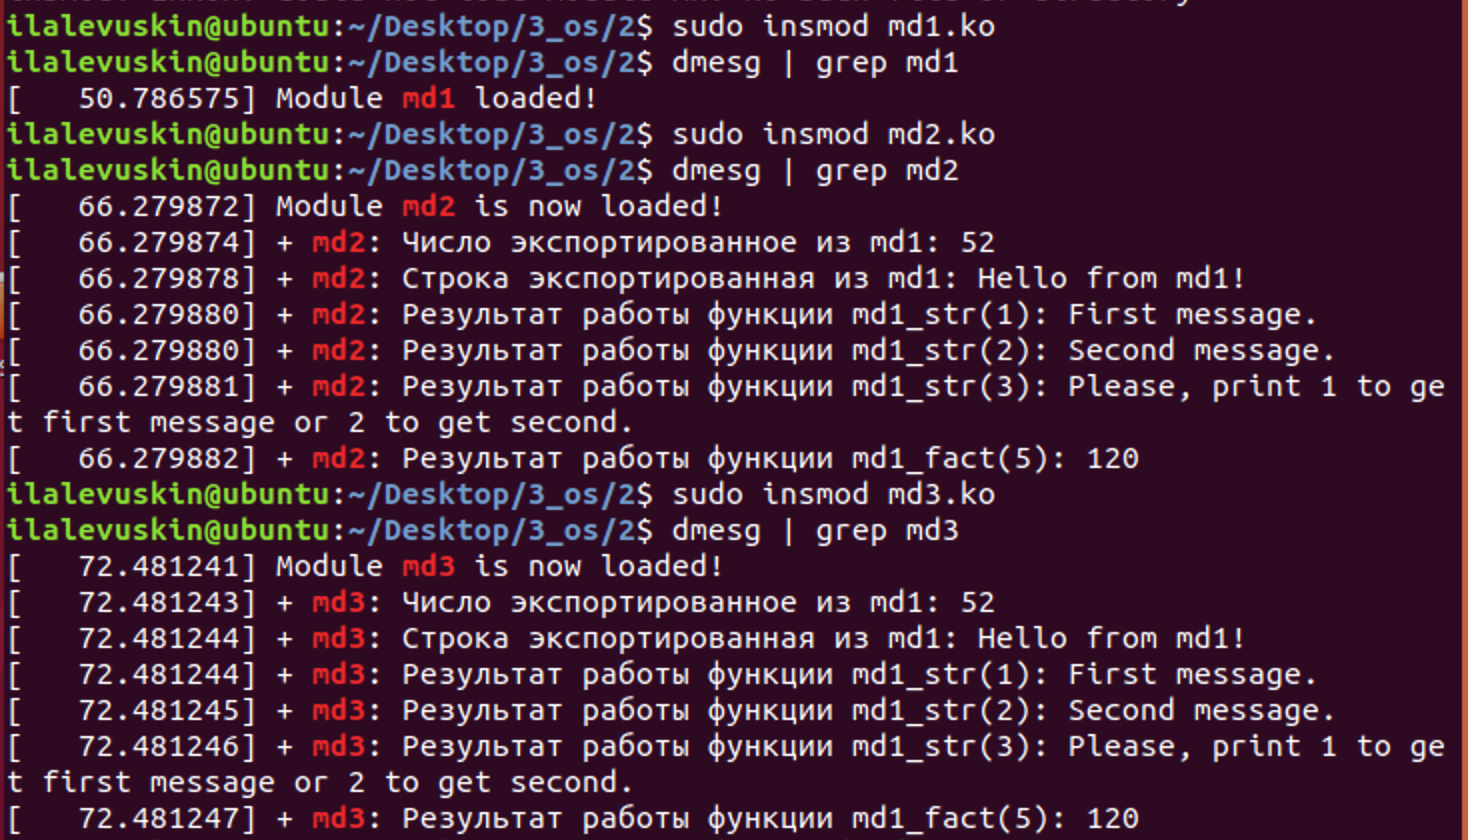
\includegraphics[scale = 0.7]{3.png}}
			\label{3}
		\end{center}
	\end{figure}
	
	Видно, что модули успешно загружены.
	
	При попытке загрузить вначале модуль <<md2>> без модуля <<md1>>, возникнет ошибка, поскольку программа не может обратиться к данным из модуля <<md1>>:
	
	\begin{figure}[h!]
		\begin{center}
			{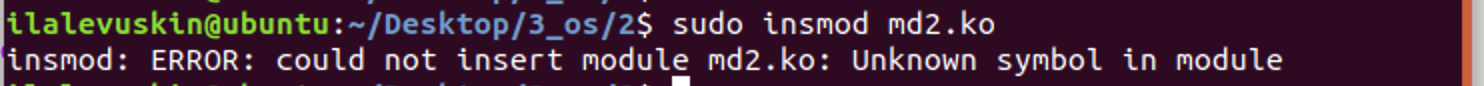
\includegraphics[scale = 0.7]{3.5.png}}
			\label{3.5}
		\end{center}
	\end{figure}

	Если же удалить из md1 экспорт данных:
	
	\begin{minted}{c}
EXPORT_SYMBOL(md1_str);
EXPORT_SYMBOL(md1_fact);

EXPORT_SYMBOL(export_char);
EXPORT_SYMBOL(export_int);
	\end{minted}
	
	И попытаться последовательно загрузить модули <<md1>>, <<md2>>, то мы также получим ошибку обращения к данным, которые недоступны:
	
	\begin{figure}[h!]
		\begin{center}
			{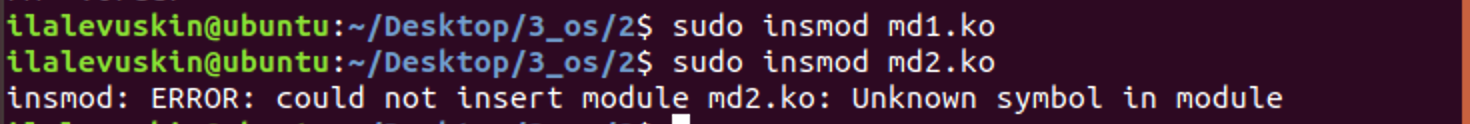
\includegraphics[scale = 0.7]{3.6.png}}
			\label{3.6}
		\end{center}
	\end{figure}
	
	Ниже продемонстрирована попытка выгрузить модули ядра, начиная с md1.
	
	\begin{figure}[h!]
		\begin{center}
			{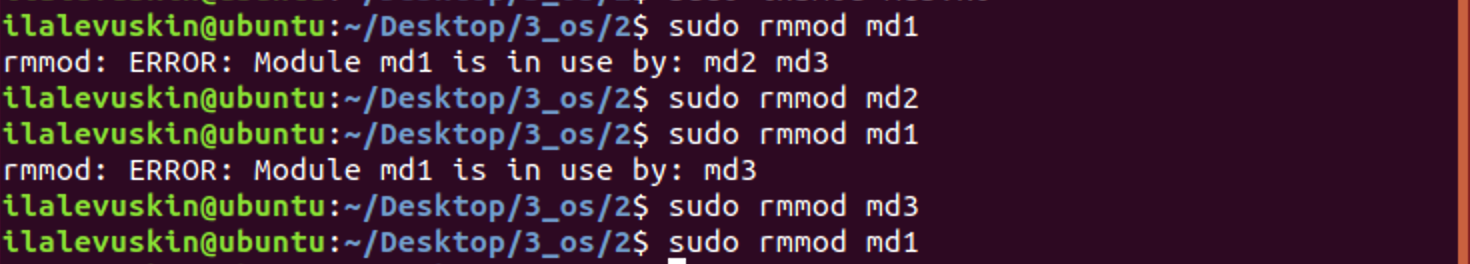
\includegraphics[scale = 0.7]{4.png}}
			\label{4}
		\end{center}
	\end{figure}
	
	Видно, что выдается сообщение об ошибке, поскольку модуль <<md1>> используется в модулях <<md2>> и <<md3>>.
	
	Таким образом, корректный порядок выгрузки модулей имеет два варианта:
	
	\begin{itemize}
		\item md2, md3, md1
		\item md3, md2, md1
	\end{itemize}
	
	
\end{document}